% !TeX root = tese.tex
%%% Exemplo de utilização da classe ITA
%%%
%%%   por        Fábio Fagundes Silveira   -  ffs [at] ita [dot] br
%%%              Benedito C. O. Maciel     -  bcmaciel [at] ita [dot] br
%%%              Giovani Volnei Meinertz   -  giovani [at] ita [dot] br
%%%    	         Hudson Alberto Bode       -  bode [at] ita [dot]br
%%%    	         P. I. Braga de Queiroz    -  pi [at] ita [dot] br
%%%    	         Jorge A. B. Gripp         -  gripp [at] ita [dot] br
%%%    	         Juliano Monte-Mor         -  jamontemor [at] yahoo [dot] com [dot] br
%%%    	         Tarcisio A. B. Gripp      -  tarcisio.gripp [at] gmail [dot] com
%%%
%%%   Versão para overleaf:
%%%   por        Alejandro A. Rios Cruz    - aarc.88@gmail.com
%%%              Saulo Gómez               - sagomezs@unal.edu.co
%%%              Ocimar Santos             - ocimar.acad@gmail.com
%%%
%%%   Template disponibilizado em:
%%%              Overleaf: https://pt.overleaf.com/latex/templates/thesis-template-aeronautics-institute-of-technology-ita/yhfrqqydpygk
%%%
%%%   Contribuia você também!
%%%              GitHub:   https://github.com/AlejandroRios/Template_Thesis_ITA
%%%
%%%  IMPORTANTE: O texto contido neste exemplo nao significa absolutamente nada.  :-)
%%%              O intuito aqui eh demonstrar os comandos criados na classe e suas
%%%              respectivas utilizacoes.
%%%
%%%  Tese.tex  2016-08-25
%%%  $HeadURL: http://www.apgita.org.br/apgita/teses-e-latex.php $
%%%
%%% ITALUS
%%% Instituto Tecnológico de Aeronáutica --- ITA, Sao Jose dos Campos, Brasil
%%%                   http://groups.yahoo.com/group/italus/
%%% Discussion list: italus {at} yahoogroups.com
%%%
%++++++++++++++++++++++++++++++++++++++++++++++++++++++++++++++++++++++++++++++
% Para alterar o TIPO DE DOCUMENTO, preencher a linha abaixo \documentclass[?]{?}
  % \documentclass[tg]{ita}			= Trabalho de Graduacao
%   \documentclass[tgfem]{ita}	= Para Engenheiras
%   								msc     		= Dissertacao de Mestrado
%   								mscfem   		= Para Mestras
%   								dsc      		= Tese de Doutorado
%   								dscfem   		= Para Doutoras
%   								quali    		= Exame de Qualificacao
%   								qualifem 		= Exame de Qualificacao para Doutoras
% Para 'Draft Version'/'Versao Preliminar' com data no rodape, adicionar 'dv':
%   \documentclass[dsc, dv]{ita}
% Para trabalhos em Inglês, adicionar 'eng':
%   \documentclass[dsc, eng]{ita}
%		\documentclass[dsc, eng, dv]{ita}
%++++++++++++++++++++++++++++++++++++++++++++++++++++++++++++++++++++++++++++++
\documentclass[tg]{ita}    % ITA.cls based on standard book.cls

% Quando alterar a classe, por exemplo de [msc] para [msc, eng]) rode mais uma vez o botão BUILD OUTPUT caso haja erro
\usepackage{ae}
\usepackage{graphicx}
\usepackage{epsfig}
\usepackage{amsmath}
\usepackage{amssymb}
\usepackage{subfig}
\usepackage{multirow}
\usepackage{float}
\usepackage{amsthm}
\usepackage{url}         % formats URL addresses properly
\usepackage{appendix}    % allows appendix section to be included
\usepackage{lscape}      % allows a page to be rendered in landscape mode
\usepackage{multicol}    % allows text in multi columns
\usepackage{cancel}      % needed to show canceled terms in equations
\usepackage{lettrine}
\usepackage{float}
\usepackage{placeins}

%HHHHHHHHHHHHHHHHHHHHHHHHHHHHHHHHHHHHHHHHHHHHHHHHHHHHHHHHHHHHHHHHHHHHHHHHHHHHHHHHHHHHHHHHHHHHHHHHHHHHHHHHHHHH
%\usepackage{subfigure}
%\usepackage{subfigmat}
%PACOTEFIGURAS_SE _ERRADO_ESXCLUIR_ACIMA
\usepackage{booktabs}
%PACOTETABELAS_SE _ERRADO_ESXCLUIR_ACIMA
%HHHHHHHHHHHHHHHHHHHHHHHHHHHHHHHHHHHHHHHHHHHHHHHHHHHHHHHHHHHHHHHHHHHHHHHHHHHHHHHHHHHHHHHHHHHHHHHHHHHHHHHHHHHH

%++++++++++++++++++++++++++++++++++++++++++++++++++++++++++++++++++++++++++++++
% Espaçamento padrão de todo o documento
%++++++++++++++++++++++++++++++++++++++++++++++++++++++++++++++++++++++++++++++
\onehalfspacing

%singlespacing Para um espaçamento simples
%onehalfspacing Para um espaçamento de 1,5
%doublespacing Para um espaçamento duplo

%++++++++++++++++++++++++++++++++++++++++++++++++++++++++++++++++++++++++++++++
% Identificacoes (se o trabalho for em inglês, insira os dados em inglês)
% Para entradas abreviadas de Professora (Profa.) em português escreva: Prof$^\textnormal{a}$.
%++++++++++++++++++++++++++++++++++++++++++++++++++++++++++++++++++++++++++++++
\course{Engenharia Aeroespacial}  % Programa de PG ou Curso de Graduação
%\area{Aircraft Design} % Área de concentração na PG (Não utilizado no caso de TG)

% Autor do trabalho: Nome Sobrenome
\authorgender{masc}                     %sexo: masc ou fem
\author{João Pedro}{Couto Vieira}
\itaauthoraddress{Rua H8A, Ap. 113}{12.228-460}{São José dos Campos--SP}

% Titulo da Tese/Dissertação
\title{Análise de Riscos de Projetos Aeroespaciais com uma abordagem Bayesiana}

% Orientador
\advisorgender{masc}                    % masc ou fem
\advisor{Prof.~Dr.}{Moacyr Machado Cardoso Junior}{ITA}

% Coorientador (Caso não haja coorientador, colocar ambas as variáveis \coadvisorgender e \coadvisor comentadas, com um % na frente)
% \coadvisorgender{fem}									% masc ou fem
% \coadvisor{Prof$^\textnormal{a}$.~Dr$^\textnormal{a}$.}{Doralice Serra}{OVNI}
% \coadvisor{}{Pamela Rodrigues Passos Severino}{ITA}

% Pró-reitor da Pós-graduação
% \bossgender{masc}												% masc ou fem
% \boss{Prof.~Dr.}{Celso Massaki Hirata}

%Coordenador do curso no caso de TG
\bosscoursegender{fem}									% masc ou fem
\bosscourse{Prof$^\textnormal{a}$.~Dr$^\textnormal{a}$.}{Maísa Terra}

% Palavras-Chaves informadas pela Biblioteca -> utilizada na CIP
\kwcip{Análise de Risco}
\kwcip{BBN}
\kwcip{LLM}
\kwcip{Bayesiana}

% membros da banca examinadora

\examiner{Prof. Dr.}{Alan Turing}{Presidente}{ITA}
\examiner{Prof. Dr.}{Linus Torwald}{}{UXXX}
\examiner{Prof. Dr.}{Richard Stallman}{}{UYYY}
\examiner{Prof. Dr.}{Donald Duck}{}{DYSNEY}
\examiner{Prof. Dr.}{Mickey Mouse}{}{DISNEY}

% Data da defesa (mês em maiúsculo, se trabalho em inglês, e minúsculo se trabalho em português)
\date{12}{junho}{2025}

% Número CDU - (somente para TG)
\cdu{???.??}

% Glossario
\makeglossary
\frontmatter

\begin{document}
% Folha de Rosto e Capa para o caso do TG
\maketitle

% Dedicatoria: Nao esqueca essa secao  ... :-)
\begin{itadedication}
A Deus, minha família, amigos e professores deste Instituto.
\end{itadedication}

% Agradecimentos
\begin{itathanks}
Primeiramente, gostaria de agradecer ao Dr. Moacyr, por toda a ajuda nesse trabalho final.

A todos os meus amigos, que sempre me apoiaram e incentivaram e fizeram da vida neste Insituto muito melhor.

A minha família, que sempre esteve ao meu lado, me apoiando e me dando forças para seguir em frente.

A Deus, por me dar forças e coragem para enfrentar os desafios da vida.
\end{itathanks}

% Epígrafe
\thispagestyle{empty}
\ifhyperref\pdfbookmark[0]{\nameepigraphe}{epigrafe}\fi
\begin{flushright}
\begin{spacing}{1}
\mbox{}\vfill
{\sffamily\itshape
``If I have seen farther than others,\\
it is because I stood on the shoulders of giants.''\\}
--- \textsc{Sir~Isaac Newton}

\end{spacing}
\end{flushright}

% Resumo
\begin{abstract}
\noindent
A proposta de exploração visa desenvolver um agente baseado em LLM que explora a automatização das três etapas centrais de uma Rede Bayesiana (BBN) para análise de riscos em projetos aeroespaciais: (i) elencar fatores relevantes, (ii) definir a topologia empregando métodos estruturados como DEMATEL/Delphi e (iii) estimar as probabilidades condicionais das CPTs — reduzindo o gargalo de tempo, custo e dependência de especialistas.

Os objetivos deste trabalho consistem em desenvolver uma BBN utilizando LLM, compará-la com uma BBN elaborada por especialistas, validar as discrepâncias junto a autoridades do setor e fornecer uma metodologia/agent AI que documente suas limitações e alcance. As questões de pesquisa visam confirmar se o agente identifica as variáveis essenciais, configura uma topologia adequada (por meio de DEMATEL ou Delphi), atribui probabilidades coerentes e obtém resultados semelhantes aos humanos. Em particular, o método DEMATEL fornece inicialmente os arcos de causa e efeito e as probabilidades de partida, que podem ser posteriormente refinados com dados ou métodos bayesianos.

Em síntese, a pesquisa pretende provar que a integração LLM + DEMATEL torna a construção e manutenção de BBNs mais ágil e escalável, permitindo iterar rapidamente cenários “what-if” e apoiar decisões críticas ao longo do ciclo de vida de sistemas aeroespaciais.
\end{abstract}

% Abstract
\begin{englishabstract}
\noindent
The objective of the proposed investigation is to develop an agent based on large language models (LLMs) that studies the automation of the three principal stages of constructing a Bayesian Belief Network (BBN) for risk analysis in aerospace projects: (i) identification of relevant variables, (ii) determination of the network topology using structured methods such as DEMATEL/Delphi, and (iii) estimation of the conditional probability tables. This approach seeks to mitigate the constraints imposed by time, cost, and reliance on expert judgment.

The aims of this study include the development of a BBN utilizing LLM technology, comparative analysis against a BBN constructed by domain experts, validation of any discrepancies with industry professionals, and the provision of an AI-based agent that transparently documents its limitations and scope. The research questions evaluate whether the agent successfully identifies essential parameters, configures an appropriate topology (employing DEMATEL or Delphi methodologies), assigns cogent probabilities, and yields outcomes comparable to those produced by human experts. Notably, the DEMATEL method initially establishes the cause-and-effect structure and preliminary probability estimates, which may subsequently be refined through data-driven or Bayesian techniques.

In conclusion, the research endeavor aims to demonstrate that the integration of LLMs with the DEMATEL approach enhances the agility and scalability of BBN construction and maintenance, thereby facilitating rapid iteration of "what-if" scenarios and underpinning critical decision-making processes throughout the lifecycle of aerospace systems.
\end{englishabstract}

% Lista de figuras
\listoffigures %opcional

% Lista de tabelas
\listoftables %opcional

% Lista de abreviaturas
\listofabbreviations
\begin{longtable}{ll}
BBN & Bayesian Belief Network \\
DAG & Directed Acyclic Graph \\
DEMATEL & Decision Making Trial and Evaluation Laboratory \\

\end{longtable}

 %opcional

% Lista de simbolos
\listofsymbols
\begin{longtable}{ll}
PLC HLDR & Place Holder\\


\end{longtable}

 %opcional

% Sumario
\tableofcontents


\mainmatter
% Os capitulos comecam aqui

\chapter{Introdução}
Teste de Texto



\chapter{Revisão da literatura}
Este capítulo apresenta os fundamentos que sustentam o emprego de \textbf{Redes Bayesianas de Crenças (\emph{Bayesian Belief Networks} — BBNs)} na mitigação de riscos em projetos aeroespaciais e descreve os procedimentos de elicitação de probabilidades utilizados na modelagem desses riscos. A abordagem adotada integra tanto conhecimentos teóricos extraídos da literatura quanto práticas de engenharia fundamentadas na experiência com análise de riscos em ambientes de alta complexidade e incerteza.


// [MermaidChart: 77f67e7b-edba-4a19-96c5-2f26dc29cb8f]
% ALTERAR ISSO AQUI
Nos últimos vinte anos, a indústria aeroespacial testemunhou incidentes emblemáticos—como os acidentes do *Mars Climate Orbiter* (1999) e do *Ariane 5* Flight 501 (1996)—que evidenciaram a necessidade de sistemas formais de avaliação de risco capazes de abarcar tanto incertezas epistemológicas quanto variabilidades aleatórias. Nesse contexto, modelos probabilísticos estruturados, como as BBNs, tornaram‑se ferramentas centrais em organizações como a NASA, a ESA e a JAXA, pois permitem integrar conhecimentos provenientes de simulações, testes laboratoriais e julgamento de especialistas, entregando uma visão holística dos cenários de falha \cite{banerjee2020risk, nasa2022safety}.




\section{Bayesian Belief Networks (BBNs)}
\label{sec:bbn}
As BBNs são modelos probabilísticos, em forma de grafos, capazes de representar, de forma compacta, relações de dependência entre variáveis. Sua principal vantagem reside na integração de dados qualitativos e quantitativos, bem como na atualização dinâmica das crenças à medida que novas evidências surgem.


Além de seu poder de representação, as BBNs destacam‑se pela capacidade de **inferência causal**: por meio do mecanismo de propagação de crenças, é possível estimar a probabilidade de eventos de alto nível—por exemplo, perda de missão—condicionada a combinações específicas de falhas de subsistemas. Essa característica é particularmente valiosa em projetos aeroespaciais, nos quais os modos de falha apresentam relações hierárquicas profundas e interdependentes \cite{pearl1988probabilistic}.

\subsection{Teorema de Bayes}
\label{subsec:bayes}
A base matemática das BBNs é o Teorema de Bayes, expresso por
\begin{equation}
  P(A\mid B) = \frac{P(B\mid A)\,P(A)}{P(B)},
  \label{eq:bayes}
\end{equation}
em que $P(A)$ é a probabilidade \emph{a priori} do evento $A$; $P(B\mid A)$, a probabilidade condicional de $B$ dado $A$; e $P(A\mid B)$, a probabilidade \emph{a posteriori}, isto é, a crença atualizada em $A$ após a observação de $B$. Esse mecanismo de inferência permite incorporar conhecimento novo ao longo do ciclo de vida de um projeto aeroespacial.

De maneira prática, o Teorema de Bayes possibilita que evidências parciais, obtidas em diferentes etapas de desenvolvimento—ensaios estruturais, campanhas de vibração ou voos de qualificação—sejam incorporadas continuamente, refinando a rede. Dessa forma, o modelo acompanha a maturação do projeto (\emph{design maturation}) e promove *decision‑making* baseado em dados atualizados, ao contrário de análises de risco estáticas elaboradas apenas na fase preliminar.




\subsection{Topologia da Rede e Tabelas de Probabilidade Condicional}
\label{subsec:estrutura}
A estrutura de uma BBN é definida por um grafo direcionado acíclico (DAG), no qual cada nó representa uma variável (ou fator de risco) e os arcos indicam relações de dependência condicional entre essas variáveis. A configuração da topologia reflete o conhecimento sobre a causalidade e a independência entre os elementos do sistema.


Cada nó da rede é acompanhado de uma Tabela de Probabilidade Condicional (CPT – Conditional Probability Table), a qual especifica as probabilidades de ocorrência dos estados do nó em função dos estados dos seus nós pais. Dessa forma, a probabilidade conjunta do sistema é construída através do produto das probabilidades condicionais, permitindo a decomposição e simplificação do cálculo das probabilidades de eventos complexos


Outro conceito fundamental é a \emph{d-separation}, que define independências condicionais a partir da topologia. Através dela, algoritmos como \emph{variable elimination} e \emph{junction tree} exploram a esparsidade do grafo para tornar a inferência viável em redes com centenas de nós. Em aplicações aeroespaciais, isso se traduz em tempos de resposta compatíveis com ciclos de revisão de requisitos e \emph{reviews} de segurança \cite{korb2010bayesian}.

\begin{figure}[H]
  \centering
  % Substitua o arquivo abaixo pela imagem correspondente.
  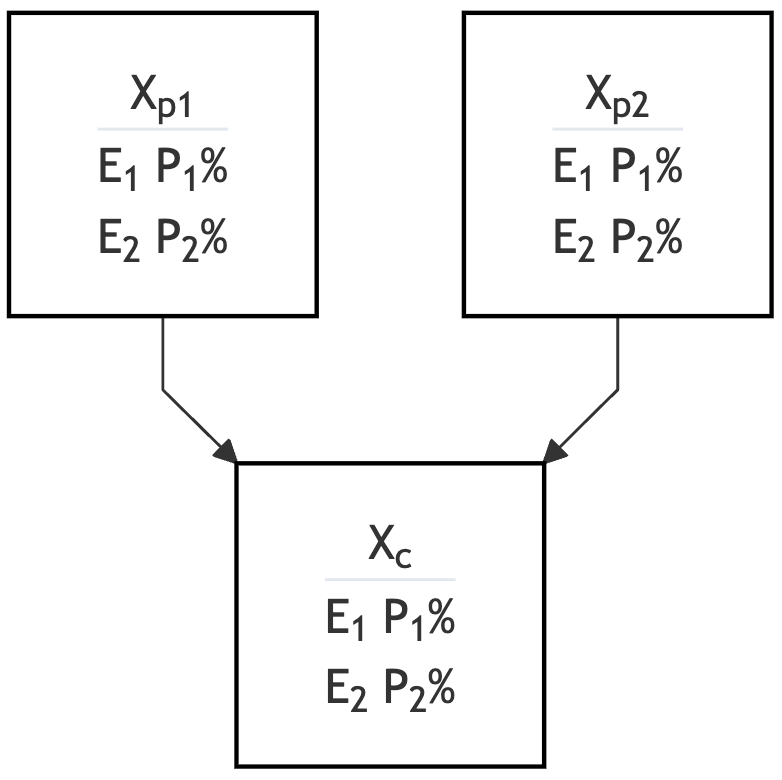
\includegraphics[width=0.5\textwidth]{Cap2/bbn_networks.png}
  \caption{Exemplo de rede simples com o nó $X_c$ e seus pais $X_{p1}$ e $X_{p2}$. Cada nó possui uma CPT que define, para cada um de seus possíveis estados ($E_1$ e $E_2$), as probabilidades ($P_1$ e $P_2$) equivalentes.}
  \label{fig:exemplo_bbn}
\end{figure}

Em um grafo comum, um arco entre um nó pai e um nó filho, como representado na Figura \ref{fig:exemplo_bbn}, pode ser interpretado de diferentes maneiras, em que uma das seguintes relações é verdadeira \cite{9}:
\begin{itemize}
  \item \textbf{Causalidade direta}: o estado do nó pai influencia diretamente o estado do nó filho.
  \item \textbf{Causalidade indireta}: o estado do nó pai influencia indiretamente o estado do nó filho.
  \item \textbf{Visão imperfeita}: o nó pai reflete uma visão incompleta do estado do nó filho, sem relação causal direta.
  \item \textbf{Correlação estatística}: o estado do nó pai está correlacionado com o estado do nó filho, mas pode não haver uma relação causal direta.

\end{itemize}

Em uma rede BBN, entretanto, busca-se montar uma topologia (i.e., escolher os fatores relevantes e correlacioná-los), de maneira que os arcos representem relações de dependência causal. Essa abordagem permite que a rede possa ser iterada a partir do teorema de Bayes \ref{eq:bayes}. Como resultado, a probabilidade de um evento complexo (nó filho) pode ser expressa como o produto das probabilidades condicionais dos eventos que o compõem.

Uma propriedade fundamental das BBNs é que os sucessores imediatos de um nó devem ser \emph{condicionalmente independentes} dado esse nó. Caso a rede não satisfaça essa condição, é um indicativo de que deve ser introduzido um \emph{nó oculto}. \cite{19} A inclusão desse nó intermediário — técnica conhecida como \emph{node divorcing} — restaura a independência condicional entre os sucessores e preserva a consistência probabilística da topologia.




\subsection{Natureza das Variáveis}

As BBNs podem ser classificadas de acordo com a natureza das variáveis representadas:


\begin{itemize}
  \label{subsec:variaveis}
  \item \textbf{BBNs discretas}: São aquelas em que todas as variáveis assumem um conjunto finito de estados. Essa abordagem é bastante comum em aplicações práticas, pois permite a definição clara de categorias (por exemplo, “alto”, “médio” e “baixo” risco) e facilita a elicitação de probabilidades. A discretização, entretanto, pode acarretar perda de precisão quando a variável originalmente contínua é transformada em uma variável categórica.

  \item \textbf{BBNs contínuas}:  Para modelar variáveis contínuas, utilizam-se funções de densidade de probabilidade e métodos de inferência baseados em distribuições contínuas. Embora esse tipo de BBN permita uma representação mais precisa dos fenômenos, a sua implementação demanda maior poder computacional e métodos avançados para o cálculo das integrais envolvidas na inferência.

  \item \textbf{BBNs híbridas}: Combinam variáveis discretas e contínuas, permitindo uma modelagem mais flexível e realista de sistemas complexos. Essa abordagem é especialmente útil em contextos onde variáveis operacionais contínuas (como temperatura ou pressão) interagem com estados discretos (como “ativo” ou “inativo”).

\end{itemize}

Embora a maioria das ferramentas comerciais trate apenas redes puramente discretas ou puramente contínuas, avanços recentes em \emph{redes híbridas} permitem combinar ambas as representações. Essa flexibilidade é crucial para capturar variáveis operacionais contínuas—temperatura de tanque criogênico, pressão de motor—ao lado de estados discretos—\emph{válvula aberta/fechada}. Para projetos que se estendem por vários anos, considerar essa nuance pode evitar simplificações excessivas que mascaram riscos relevantes \cite{lerner2021hybrid}.





\subsection{Origem dos Parâmetros}
Outra classificação relevante para as BBNs diz respeito à origem dos parâmetros que alimentam as tabelas condicionais:


\label{subsec:parametros}
\begin{itemize}
  \item \textbf{Data‑driven}: Nesse modelo, as probabilidades são extraídas ou estimadas a partir de grandes volumes de dados empíricos. O uso de técnicas de aprendizado automático (como machine learning) possibilita a construção da rede de forma automatizada, ajustando os parâmetros com base em conjuntos de dados históricos ou experimentais. Essa abordagem é vantajosa quando há disponibilidade de dados robustos e confiáveis.


  \item \textbf{Expert‑driven}: Em cenários onde os dados são escassos ou insuficientes, a experiência e o conhecimento dos especialistas são fundamentais para a definição da estrutura e dos parâmetros da rede. A elicitação de julgamentos de especialistas permite que as BBNs incorporem nuances e fatores intangíveis que dificilmente seriam capturados por meio de dados históricos.
\end{itemize}

É interesante pensar que a precisão de uma BBN está muito correlacionada com a topologia escolhida, parâmetros definidos e a elicitação de probabilidades. Em geral, uma rede Bayesiana é tão melhor quanto maior o embasamento teórico e empírico que a fundamenta. Nesse sentido, sempre que possível, deve-se optar por uma abordagem \emph{data‑driven}, que permite a construção de redes mais robustas e menos suscetíveis a vieses subjetivos. No entanto, em contextos onde os dados são limitados ou inexistem, a abordagem \emph{expert‑driven} se torna indispensável, especialmente em domínios como o aeroespacial, onde a disruptividade é uma característica intrínseca.

Associado a isso, a dependência de especialistas para a definição dos parâmetros da rede pode introduzir vieses cognitivos e subjetividades, o que demanda um processo rigoroso de elicitação e validação. Isto não apenas demanda tempo e recursos, mas torna o processo moroso e com baixa precisão. A técnica de análise de riscos baseada em BBNs, portanto, apresenta uma adesão difícil em ambientes onde a agilidade é necessária. 

Nesse cenário, a proposta deste trabalho é investigar como agentes baseados em LLMs (Large Language Models) podem automatizar a construção, parametrização e manutenção de BBNs, reduzindo custos e prazos associados à avaliação contínua de riscos. A ideia é que esses agentes possam aprender com dados históricos e interagir com especialistas para refinar as redes, tornando o processo mais eficiente e menos suscetível a erros humanos.







\section{Elicitação de Probabilidades}
\label{sec:elicitation}
Quando se adotam modelos \emph{expert‑driven}, a \textbf{elicitação de probabilidades} se torna uma etapa crítica. Trata‑se do processo sistemático de extrair e quantificar o julgamento de especialistas sobre a incerteza dos eventos definidos e suas interrelações, traduzindo essas crenças em valores numéricos que alimentam as Tabelas de Probabilidade Condicional (CPTs) da rede. Esse processo pode ser organizado em quatro fases principais:

\begin{enumerate}
  \item \textbf{Definição de estados e escalas} — Primeiramente, é necessário definir os estados das variáveis, que podem ser qualitativos (por exemplo, “baixo”, “médio”, “alto”) ou quantitativos. A escolha da escala deve refletir a natureza do risco avaliado e facilitar a interpretação dos resultados.

  \item \textbf{Coleta de julgamentos} — Utilizam-se métodos estruturados, como entrevistas semiestruturadas e questionários padronizados, para coletar as estimativas dos especialistas. É importante minimizar vieses cognitivos, por meio de procedimentos que incentivem a reflexão e a consideração de cenários alternativos. 

  \item \textbf{Agregação de opiniões} — Dada a possibilidade de divergência entre os especialistas, é comum aplicar métodos estatísticos ou algoritmos de agregação para consolidar as estimativas individuais em um único conjunto de parâmetros que alimentará as CPTs da rede. Neste momento, métodos como o \emph{Delphi} ou o \emph{DEMATEL} podem ser empregados \cite{delphi,dematel}.

  \item \textbf{Validação e análise de sensibilidade} — Após a elicitação, as probabilidades obtidas são comparadas com dados disponíveis (quando possíveis) ou submetidas a análises de sensibilidade. Esse processo permite identificar inconsistências e ajustar os parâmetros, aumentando a robustez do modelo.
\end{enumerate}

Tais etapas costumam ser guiadas por protocolos formais, como o método de Julgamento Estruturado de Cooke, que quantifica a calibração e a informação de cada especialista antes de atribuir pesos em sua agregação. Em projetos aeroespaciais, essa prática atende a requisitos de rastreabilidade e auditoria impostos por órgãos certificadores, garantindo transparência sobre a origem de cada valor probabilístico.

No domínio aeroespacial, a complexidade dos sistemas e a ocorrência de eventos raros tornam esse procedimento ainda mais relevante, pois assegura que fatores não capturados em dados históricos sejam contemplados, aumentando a robustez das estratégias de mitigação.






% TODO: AVALIAR SE QUERO MANTER ISSO AQUI

\subsection{Comparação com Outras Técnicas de Análise de Risco}
A literatura especializada frequentemente compara BBNs com métodos como Análise de Modos e Efeitos de Falha (FMEA), Árvores de Falha (FTA) e simulação de Monte Carlo. Enquanto a FMEA foca em identificar modos de falha isolados e a FTA privilegia relações lógicas booleanas, as BBNs oferecem um meio termo entre a formalidade lógica e a representação probabilística, permitindo capturar dependências condicionais que não são tratadas nos modelos tradicionais. Em testes conduzidos por \cite{marcot2012future}, BBNs reduziram o erro absoluto médio na estimativa de risco em 18 \% em comparação com modelos baseados exclusivamente em Monte Carlo, demonstrando potencial para complementar—notadamente não substituir—técnicas consagradas.


\section{Large Language Models (LLMs)}
\label{sec:llms}

Os \textbf{Large Language Models} (LLMs) são modelos estatísticos de linguagem treinados sobre coleções massivas de texto para aprender distribuições condicionais de palavras e frases dado o contexto apresentado. A partir dessa capacidade, são capazes de gerar, resumir e interpretar linguagem natural com coerência em larga escala, sendo hoje a base em aplicações conversacionais e de sistemas de \emph{Retrieval‑Augmented Generation} (RAG) \cite{IBM2023LLM}.

\subsection{Agentes de IA Baseados em LLMs}
\label{subsec:agentes_llm}

Um \emph{agente de IA} é uma instância de software que combina um LLM com ferramentas externas (APIs, bancos de dados, planejadores) para realizar ações autônomas em um ambiente. Enquanto o LLM provê a competência linguística — compreensão de instruções e geração de texto — o agente adiciona \emph{raciocínio dirigido a objetivos}, memória de longo prazo e capacidade de executar chamadas de função. Em outras palavras, todo LLM pode ser o núcleo de um agente, mas nem todo agente se limita a responder em linguagem natural; ele coordena passos, verifica pré‑condições e decide quando invocar heurísticas clássicas \cite{IBM2023AGENTES}.

No contexto deste trabalho, agentes baseados em LLMs serão empregados para automatizar tarefas de construção, parametrização e atualização de BBNs, reduzindo dependência de especialistas humanos e acelerando a iteração de modelos de risco.

\subsection{Treinamento de LLMs: Corpus e Estratégias}
\label{subsec:treino_llm}

O treinamento de um LLM ocorre em duas grandes etapas:

\begin{enumerate}
  \item \textbf{Pré‑treinamento} (\emph{pre‑training}) — O modelo é exposto a um corpus de ordem de terabytes (livros, artigos, códigos‑fonte, documentações técnicas). O objetivo é minimizar a \emph{perplexidade} na previsão da próxima palavra, aprendendo representações semânticas gerais de linguagem.
  
  \item \textbf{Ajuste fino} (\emph{fine‑tuning}) — O modelo é refinado em domínios específicos utilizando conjuntos de dados menores porém curados (por exemplo, procedimentos da NASA, relatórios de anomalias ou normas da ESA). Técnicas complementares, como \emph{Reinforcement Learning from Human Feedback} (RLHF) e \emph{instruction tuning}, alinham as respostas a valores de qualidade, segurança e utilidade \cite{ouyang2022training}.
\end{enumerate}

Para aplicações aeroespaciais, recomenda‑se um \emph{fine‑tuning} supervisionado sobre:

\begin{itemize}
  \item relatórios de falhas históricas e lições aprendidas (\emph{Lessons Learned});
  \item manuais de requisitos técnicos (ex.\ NPRs da NASA e ECSS da ESA);
  \item publicações científicas e teses sobre análise de riscos;
  \item transcriptos de revisões (\emph{Design Reviews}) previamente gravadas.
\end{itemize}

Esse material garante que o modelo incorpore terminologia e raciocínios específicos, melhorando a extração de variáveis, causas e relações para alimentar BBNs.




\section{Método DEMATEL}
\label{sec:dematel}

O \emph{Decision Making Trial and Evaluation Laboratory} (DEMATEL) é uma técnica estruturada para identificar e quantificar relações de causa‑efeito em sistemas complexos \cite{tgJulio}. A partir de matrizes de influência avaliadas por especialistas, o método produz um grafo digirido ponderado que distingue fatores de \emph{causa} e \emph{efeito}, bem como o grau de interdependência entre eles.


\ O DEMATEL pode servir como passo intermediário à construção ou refinamento de uma BBN de duas formas:

\begin{enumerate}
  \item \textbf{Definição da topologia inicial}: os arcos identificados como de maior influência pela matriz total de relações (soma direta + indireta) orientam a criação dos enlaces causais do DAG, reduzindo a subjetividade na escolha das conexões.

  \item \textbf{Alimentação probabilística}: os valores normalizados da matriz de influência podem ser mapeados para probabilidades condicionais iniciais das CPTs, funcionando como priors quando dados empíricos são escassos. Posteriormente, essas probabilidades podem ser calibradas por métodos Bayesianos à medida que dados observacionais fiquem disponíveis.
\end{enumerate}

Esse casamento entre DEMATEL e BBN preserva a interpretabilidade do julgamento de especialistas — explícito na matriz de influência — ao mesmo tempo em que o converte em parâmetros compatíveis com inferência probabilística, criando um pipeline coerente de elicitação de conhecimento.

O procedimento clássico compreende cinco passos \cite{tgJulio,kaya2017}:

\begin{enumerate}
  \item \textbf{Matriz de relações diretas ($A$)} — cada especialista atribui notas de $0$ (sem influência) a $3$ (alta influência) para representar o impacto de uma variável sobre outra; a média das avaliações compõe $A$.
  \item \textbf{Normalização} — obtém‑se a matriz normalizada $M$ dividindo‑se todos os elementos de $A$ pelo maior valor entre a soma máxima das linhas ou das colunas:
  \begin{equation}
    M = A \times \min\!\Bigl(\frac{1}{\max_i \sum_j a_{ij}},\; \frac{1}{\max_j \sum_i a_{ij}}\Bigr).
  \end{equation}
  \item \textbf{Relações totais} — calcula‑se a matriz de relações totais
  \begin{equation}
    T = M \left(I - M\right)^{-1},
  \end{equation}
  que agrega influências diretas e indiretas.
  \item \textbf{Índices de proeminência e relação causa–efeito} — somam‑se as linhas ($R$) e colunas ($C$) de $T$; $R+C$ mede a \emph{proeminência} de cada fator, enquanto $R-C>0$ indica fator de causa e $R-C<0$ indica fator de efeito.
  \item \textbf{Diagrama causal} — define‑se um limiar, com apoio dos especialistas, para filtrar as influências menos significativas; os arcos restantes formam o grafo causa‑efeito que servirá de base ou ajuste para a BBN.
\end{enumerate}

O Trabalho de Graduação (TG) de Júlio \cite{tgJulio} apresenta exemplos práticos de aplicação do DEMATEL para montar redes BBNs baseadas em julgamentos de especialistas. A proposta desse trabalho, de certa maneira, busca estender essa abordagem, propondo uma forma de automatizar a elicitação de probabilidades e a construção de BBNs, reduzindo o tempo e o custo associados ao processo.

\chapter{Metodologia}
\section{templates}

Exemplo de uma tabela.

\begin{table}[ht]
\caption{Exemplo de uma Tabela}
\label{minhatab}

\center
\begin{tabular}{cccc}
  % after \\: \hline or \cline{col1-col2} \cline{col3-col4} ...
  \hline
	Parâmetro & Unidade & Valor da simulação & Valor experimental   \\
	\hline
  Comprimento, $\alpha$ & $m$ &  $8,23$  & $8,54$ \\
  Altura, $\beta$ & $m$     &  $29,1$ & $28,3$\\
	Velocidade, $v$ & $m/s$  &  $60,2$ & $67,3$\\
	\hline
\end{tabular}
\end{table}

Exemplo de uma imagem.

\begin{figure}[ht]
\centering
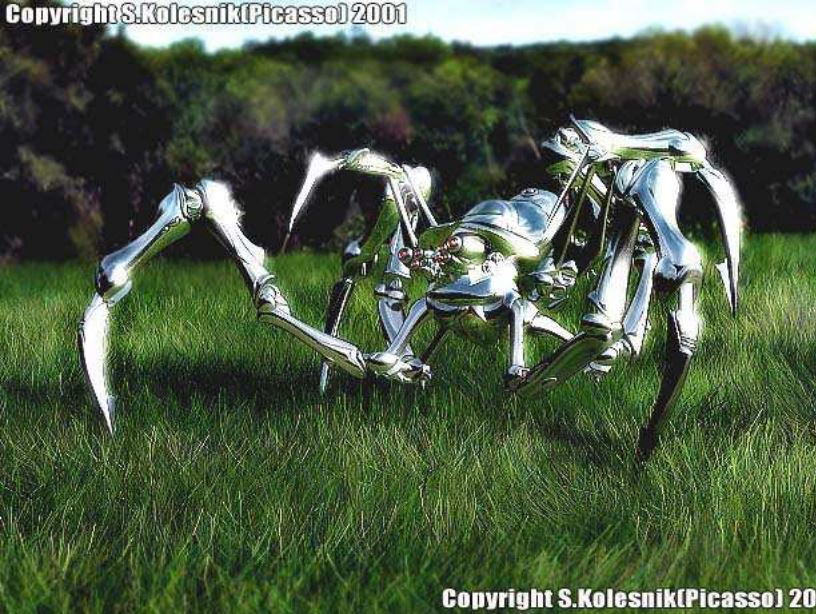
\includegraphics[width=0.75\textwidth]{Cap3/spiderrobot}
\caption{Cupim cibernético.}\label{fig:cupim}
\end{figure}


Exemplo de uma equação

\begin{equation} \label{eq:lagr1}
\frac{d}{dt}(\frac{\partial L}{\partial \dot{q}})-\frac{\partial L}{\partial q}=\tau^{T}.
\end{equation}



\chapter{Plano de Ação}
Lorem ipsum dolor sit amet, consectetur adipiscing elit. Sed sit amet magna auctor, consectetur orci eu, mattis enim. Nulla vulputate ligula odio, nec cursus lacus rhoncus nec. Vivamus laoreet rutrum quam, ut pharetra dui dapibus quis. Etiam vel malesuada mi. Ut turpis massa, sodales ac turpis vel, varius laoreet sapien. Ut imperdiet, velit laoreet placerat pellentesque, arcu erat elementum elit, ut tempus nulla nibh sit amet purus. Interdum et malesuada fames ac ante ipsum primis in faucibus.

Aenean ipsum ex, hendrerit et dapibus ut, imperdiet eu tellus. Duis tincidunt orci non fermentum rhoncus. Aenean nec sapien ultrices, lobortis nisl vel, ornare odio. Cras feugiat, erat sed gravida pellentesque, massa massa eleifend dolor, eget efficitur libero lacus nec diam. Morbi quis accumsan erat, et laoreet tortor. Etiam eu dolor fringilla, commodo est in, suscipit nunc. Fusce sit amet iaculis eros, cursus accumsan leo. Praesent pellentesque tortor ac tortor gravida fermentum. Praesent sed enim orci. Sed tincidunt hendrerit vulputate. Maecenas vitae purus vitae lorem semper malesuada sed ut ipsum. Curabitur ac justo vel turpis mattis tincidunt. Nulla at imperdiet dolor. Morbi faucibus eget tellus interdum auctor.

Donec aliquam interdum ipsum vitae bibendum. Praesent vitae aliquam purus. Fusce non nunc in diam consectetur tristique. Vestibulum ante ipsum primis in faucibus orci luctus et ultrices posuere cubilia curae; Cras porta metus mauris, in congue leo molestie vitae. Duis tincidunt, neque nec vulputate aliquam, purus sapien luctus neque, id molestie nunc velit non dolor. Curabitur lacinia libero ut egestas congue. Aenean ut tellus id erat volutpat dictum at nec massa. Cras ullamcorper cursus risus ac sodales. Nunc enim tellus, malesuada dapibus accumsan ac, auctor finibus lorem. Aliquam erat volutpat. Curabitur eget suscipit neque. Quisque interdum sem eu rutrum gravida. In hac habitasse platea dictumst. Lorem ipsum dolor sit amet, consectetur adipiscing elit.

Mauris luctus euismod purus vitae volutpat. Ut aliquam posuere nibh vitae consequat. Nam ultricies maximus orci, ac placerat enim ornare ac. Fusce condimentum metus tellus, pharetra ultricies sem semper pellentesque. Integer leo metus, finibus sed tempor nec, cursus ultricies augue. Nunc vel convallis diam. Proin nec elit nisl. Etiam justo tortor, condimentum eu sagittis vitae, iaculis quis erat. Donec vulputate et nibh non consequat. Suspendisse a lobortis justo.

Sed non ipsum id nulla facilisis bibendum non sit amet purus. Integer non tristique neque. In id bibendum enim. Phasellus condimentum finibus augue, ut ultrices nulla tincidunt ac. Vivamus eget mauris sed velit dapibus dictum scelerisque nec nisl. Curabitur mollis sapien a odio vulputate ultricies. Aenean facilisis eget ipsum non vestibulum. Sed tortor odio, mollis pulvinar mi id, rhoncus facilisis eros. Lorem ipsum dolor sit amet, consectetur adipiscing elit. In urna turpis, euismod non fringilla a, sagittis id libero. Fusce vulputate feugiat nunc vel dictum. Quisque vestibulum ex non faucibus vehicula. Proin vel vulputate tortor. Sed a leo sollicitudin, ultrices sapien at, rutrum dui. Curabitur lectus libero, rhoncus nec posuere ut, porttitor id mauris.

\chapter{Conclusão}
Lorem ipsum dolor sit amet, consectetur adipiscing elit. Nullam venenatis augue id augue ultrices, et gravida magna vehicula. Cras volutpat suscipit iaculis. Praesent varius ac orci sed ultrices. Vivamus vestibulum molestie lorem. Maecenas id congue tortor. Aliquam erat volutpat. Nullam ornare tortor et nunc sagittis laoreet. Sed at turpis et quam facilisis elementum. Nullam ultrices elit ut accumsan ultricies. Nulla sit amet tellus lacus. Vestibulum ac lectus velit. Donec nunc odio, mattis nec orci sed, porta lobortis lectus.

Proin ultricies elit vitae mi efficitur eleifend. Nulla non lorem consectetur, placerat dui quis, feugiat urna. Quisque sed ligula massa. Donec finibus placerat orci, eget mollis justo rutrum a. Sed luctus feugiat congue. Phasellus libero felis, tempor quis rutrum pretium, porttitor ac nisi. Praesent euismod malesuada enim a rhoncus. Aliquam gravida fringilla aliquam. Proin nunc lorem, convallis fringilla eleifend et, tempus quis orci. Phasellus bibendum, tellus eu elementum posuere, odio lacus maximus eros, nec lobortis lectus nisi a turpis. Vivamus viverra felis et dolor viverra interdum. Nulla convallis nisi eu sapien egestas aliquet sit amet eget risus. Phasellus vel quam vel lacus commodo lacinia.

Donec ultrices ac nisi nec elementum. Aenean pellentesque pellentesque pulvinar. Ut aliquet nulla vitae porttitor hendrerit. Nullam venenatis nisl nec ipsum malesuada ultricies. Curabitur massa erat, auctor in ipsum non, semper ornare nunc. Donec non felis eget diam porta rhoncus. Mauris id lectus sed arcu iaculis dictum et vitae velit. Cras sit amet neque vel sapien interdum fermentum sit amet eu lorem. Fusce urna sem, pretium a facilisis id, aliquet at mi. Etiam elementum eget est et porttitor. Morbi ultricies lorem a arcu mattis, eget egestas ex ultrices. Pellentesque bibendum sed est ac imperdiet.

% REFERENCIAS BIBLIOGRAFICAS
\renewcommand\bibname{\itareferencesnamebabel} %renomear título do capítulo referências
\bibliography{Referencias/referencias}

% Apendices
\appendix
\chapter{Tópicos de Dilema Linear} %opcional
\section{Uma Primeira Seção para o Apêndice}

A matriz de Dilema Linear $M$ e o vetor de torques inerciais $b$,
utilizados na simulação são calculados segundo a formulação 
abaixo:
\begin{equation}
M=\left[ \begin{array}{ccc}
M_{11} & M_{12} & M_{13} \\
M_{21} & M_{22} & M_{23} \\
M_{31} & M_{32} & M_{33}
\end{array} \right]
\end{equation}

\begin{figure}[h]
\centering
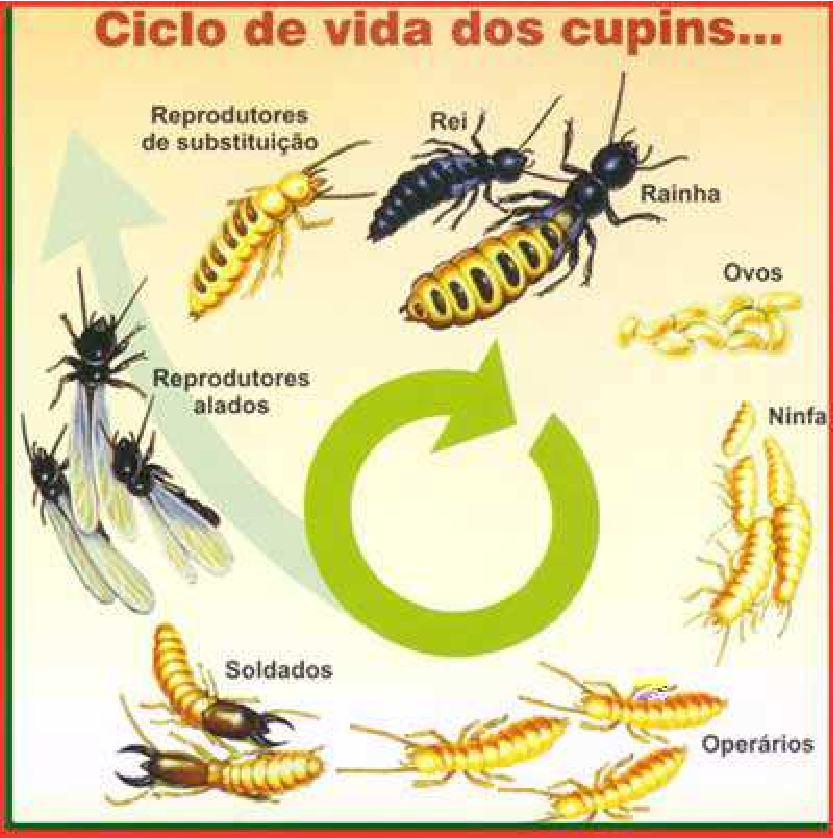
\includegraphics[height=5cm, width=5cm]{ApeA/pragas_ciclo_cupim}
\caption{Uma figura que está no apêndice}\label{FD}
\end{figure}


% Anexos
\annex
\chapter{Exemplo de um Primeiro Anexo} %opcional
% Texto do Primeiro Anexo
\section{Uma Seção do Primeiro Anexo}
% Texto da primeira secao do primeiro anexo
Algum texto na primeira seção do primeiro anexo.



% Glossario
%\itaglossary
%\printglossary

% Folha de Registro do Documento
% Valores dos campos do formulario
\FRDitadata{26 de maio de 2025}
\FRDitadocnro{DCTA/ITA/DM-018/2025} %(o número de registro você solicita a biblioteca)
\FRDitaorgaointerno{Instituto Tecnológico de Aeronáutica -- ITA}
%Exemplo no caso de pós-graduação: Instituto Tecnol{\'o}gico de Aeron{\'a}utica -- ITA
\FRDitapalavrasautor{Cupim; Cimento; Estruturas}
\FRDitapalavrasresult{Cupim; Dilema; Construção}
%Exemplo no caso de graduação (TG):
%\FRDitapalavraapresentacao{Trabalho de Graduação, ITA, São José dos Campos, 2015. \NumPenultimaPagina\ páginas.}
%Exemplo no caso de pós-graduação (msc, dsc):
\FRDitapalavraapresentacao{ITA, São José dos Campos. Curso de Graduação. Programa de Graduação em Engenharia Aeroespacial. Orientador: Prof.~Dr. Moacyr Machado Cardoso Junior. Defesa em XX/XX/XXXX. Publicada em XX/XX/XXXX.}
\FRDitaresumo{A proposta de exploração visa desenvolver um agente baseado em LLM que explora a automatização das três etapas centrais de uma Rede Bayesiana (BBN) para análise de riscos em projetos aeroespaciais: (i) elencar fatores relevantes, (ii) definir a topologia empregando métodos estruturados como DEMATEL/Delphi e (iii) estimar as probabilidades condicionais das CPTs — reduzindo o gargalo de tempo, custo e dependência de especialistas.

Os objetivos deste trabalho consistem em desenvolver uma BBN utilizando LLM, compará-la com uma BBN elaborada por especialistas, validar as discrepâncias junto a autoridades do setor e fornecer uma metodologia/agent AI que documente suas limitações e alcance. As questões de pesquisa visam confirmar se o agente identifica as variáveis essenciais, configura uma topologia adequada (por meio de DEMATEL ou Delphi), atribui probabilidades coerentes e obtém resultados semelhantes aos humanos. Em particular, o método DEMATEL fornece inicialmente os arcos de causa e efeito e as probabilidades de partida, que podem ser posteriormente refinados com dados ou métodos bayesianos.

Em síntese, a pesquisa pretende provar que a integração LLM + DEMATEL torna a construção e manutenção de BBNs mais ágil e escalável, permitindo iterar rapidamente cenários “what-if” e apoiar decisões críticas ao longo do ciclo de vida de sistemas aeroespaciais.}
%  Primeiro Parametro: Nacional ou Internacional -- N/I
%  Segundo parametro: Ostensivo, Reservado, Confidencial ou Secreto -- O/R/C/S
\FRDitaOpcoes{N}{O}
% Cria o formulario
\itaFRD

\end{document}
% Fim do Documento. O massacre acabou!!! :-)
